\subsection{Simulation}

The implementation scheme is shown in Figure \ref{fig:block}.

\begin{figure}[H]
    \centering
    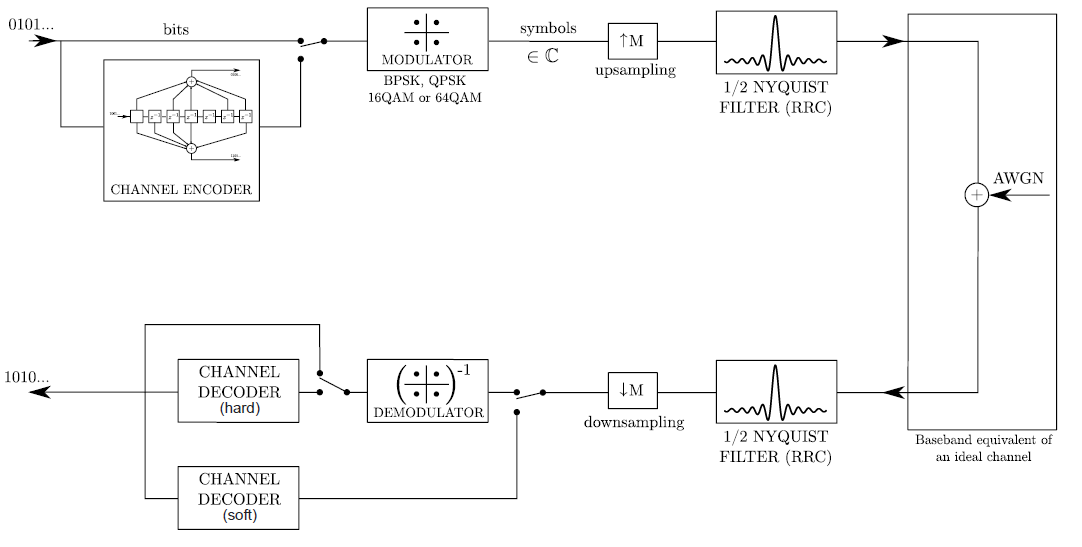
\includegraphics[width = .9\textwidth]{fig/block.png}
    \caption{Block scheme of the ideal channel}
    \label{fig:block}
\end{figure}

The various components of the communication chain are detailed hereafter. The channel encoder is not yet implemented, and the symbols mapping/demapping were provided.

\subsubsection{Halfroot Nyquist filter}

After the mapping, the complex symbols are convolved with a root raised-cosine filter. It allows to limit the communication bandwidth, as illustrated in Figure \ref{fig:filter} where the PSD of the symbol stream are shown before and after filtering, with a rolloff factor $\beta$ of $0.3$. The symbol frequency was fixed to 2 \si{\mega \hertz}, which translates to a cutoff frequency of 1 \si{\mega \hertz}.

\begin{figure}[H]
\centering
    \includegraphics{fig/filter.tex}
     \caption{PSD of the symbol stream at the transmitter before and after filtering}
    \label{fig:filter}
\end{figure}

At the receiver side, the stream is convolved again with the matched filter, forming a Nyquist filter and maximizing the SNR. The Nyquist filter allows to cancel the ISI in the sense that it reduces to a Dirac pulse when sampled at the symbol frequency, as shown in Figure \ref{fig:isi}. Hence, no symbol of the symbol stream overlaps with the current received symbol.

\begin{figure}[H]
\centering
    \includegraphics{fig/isi.tex}
     \caption{Illustration of the cancellation of ISI by the Nyquist halfroot filter}
    \label{fig:isi}
\end{figure}


\subsubsection{Noise addition}

The channel is corrupted by Additive White Gaussian Noise (AWGN), which is simulated using its baseband equivalent representation. The channel was simulated for various SNR (defined with respect to the bit energy) and various modulation schemes, and the results are plotted in Figure \ref{fig:ber}. The simulations confirm the theoretical results.


\begin{figure}[H]
\centering
    \includegraphics{fig/ber2.tex}
    \caption{Bit error rate as a function of the SNR for various modulations. The full lines correspond to the theoretical curves and the dots to the simulation.}
    \label{fig:ber}
\end{figure}

As expected, more energy is required to have the same BER when the constellation size is increased. It is worth noting that the worst BER value that could be achieved is 0.5, corresponding to a random choice of the binary values. Moreover, the BER curves for 2-PAM and 4-QAM are superposed because a 4-QAM modulation can be seen as two 2-PAM modulations in quadrature.



\newpage
\subsection{Questions}

\subsubsection{Questions regarding the simulation}

\paragraph{It is proposed to use the baseband equivalent model of the AWGN channel. Would it be possible to live with a bandpass implementation of the system ?} \mbox{}

The baseband model allows to implement the simulations regardless of the carrier frequency. If the system were simulated in bandpass, the required sampling frequency would be extremely high and unrealistic.

\paragraph{How do you choose the sample rate in Matlab ?} \mbox{}

The sampling rate should be at least twice as high as the symbol frequency. It will be increased further when simulating the sample time shift in the third step.

\paragraph{How do you make sure you simulated the desired $E_b/N_0$ ratio ?} \mbox{}

First the energy of a bit is evaluated, then the noise power is computed in order to obtain the desired $E_b/N_0$ ratio. The energy of the bit $E_b$ is given by

\begin{equation*}
    E_b = \frac{T_{samp}}{2 N_{bits}} \sum_{n} {\left| s \left[ n \right] \right|}^2
\end{equation*}

Then $N_0$ can be chosen according to the wanted SNR and the noise is added to the symbols using the baseband representation :

\begin{equation*}
    r \left[ k \right] = \sqrt{N_0 f_{samp}} \left\{ \mathcal{N}(0,1) + j \mathcal{N}(0,1) \right\}  
\end{equation*}

The square root is present because of the baseband representation of the noise. Indeed, the computed power is equally distributed between the real and imaginary parts of the noise.

\paragraph{How do you choose the number of transmitted data packets and their length ?} \mbox{}

A rule of thumb is to send $10^{n+2}$ bits of data in order to reliably observe of BER of $10^{-n}$ as it corresponds to 100 detected errors. Moreover, the total number of bits should be a multiple of the number of bits per symbol used in the modulation scheme. The Figure \ref{fig:ber} was realised by sending around $10^8$ bits of data.

\subsubsection{Questions regarding the communication system}

\paragraph{Determine the supported (uncoded) bit rate as a function of the physical bandwidth.} \mbox{}

The bit rate $R$ is given by $R = \frac{log_2 (M)}{T}$ where $M$ is the number of symbols and $T$ is the symbol duration. The Nyquist filtering yields a relationship between the symbol duration and the bandwidth, $\Delta f = 2/T$ (this can be seen on Figure \ref{fig:filter} where T = 0.5 \si{\micro \second} and $\Delta f = 2$ \si{\mega \hertz}). This gives:

\begin{equation*}
    R = \frac{log_2 (M) \ \Delta f}{2}
\end{equation*}

\paragraph{Explain the trade-off communication capacity/reliability achieved by varying the constellation size.} \mbox{}

As detailed in the previous question, increasing the constellation size (the number of bits transmitted per symbol $M$) allows to increase the bit rate. However, the minimum euclidean distance between the symbols in the constellation size decreases, which causes the error probability to increase. As a result, to achieve a similar BER, more energy is required when the constellation size increases but the bit rate also increases.

\paragraph{Why do we choose the halfroot Nyquist filter to shape the complex symbols ?} \mbox{}

The halfroot Nyquist filter allows to limit the communication bandwidth (it is more spectrally efficient than the plain rectangular window) and allows to cancel ISI.

\paragraph{How do we implement the optimal demodulator? Give the optimization criterion.} \mbox{}

The optimal demodulator is implemented 	as a bank of K filters matched to the basis functions of the modulation scheme: 

\begin{equation*}
	h_i(t) := s_i(-t) \hspace{1cm}  i=1,...,K
\end{equation*}

The outputs to such filters are the autocorrelations between the input signal and the basis functions. The filters are mathematically equivalent to a bank of K correlators. The optimisation criterion is the maximisation of the SNR at the output. It is realized by the matched filters, and the SNR will be equal to $\frac{2\mathcal{E}}{N_0}$.

\paragraph{How do we implement the optimal detector? Give the optimization criterion.} \mbox{}

There exist two possible optimization criteria for the detector. First, the maximum a posteriori (MAP) criterion, which minimises the error probability by exploiting the knowledge of the a priori probabilities $p(\underline{s}_m)$ and the conditional probabilities $p(\underline{r}|\underline{s}_m)$, where $\underline{r}$ is the observation. It selects the symbol which is the most likely to have been sent, knowing that we observed $\underline{r}$.
	
	\begin{equation*}
		\underline{\tilde{s}}^{\text{MAP}}_m = \underset{\underline{s}_m}{\text{max}} \ p(\underline{s}_m |\underline{r}) \stackrel{\text{Bayes}}{=}
		\underset{\underline{s}_m}{\text{max}} \ p(\underline{r} |\underline{s}_m) p(\underline{s}_m)
	\end{equation*}
	
The maximum likelihood criterion is equivalent to the MAP criterion when all the M symbols are equally probable, so that $p(\underline{s}_m) = 1/M$ is constant and can be dropped when maximizing the probabilities.
	
	\begin{equation*}
		\underline{\tilde{s}}^{\text{ML}}_m = \underset{\underline{s}_m}{\text{max}} \ p(\underline{r} |\underline{s}_m) 
	\end{equation*}
	
The ML criterion determines what symbol is the most likely to have produced the received signal by selecting the symbol which has the lowest euclidean distance to the received symbol.

